\documentclass{../exhibit}

\title{Mazes of Insanity}

%% Font
\usepackage{imfellEnglish}
\usepackage[T1]{fontenc}
\raggedright

\usepackage{background}

\backgroundsetup{
scale=1,
color=black,
opacity=0.4,
angle=0,
contents={%
  \includegraphics[height=\paperheight]{mapBackground.jpg}%%https://upload.wikimedia.org/wikipedia/commons/8/81/Nautical_chart_of_the_West_Indies_1797.jpg
  }%
}




%% For the context
%% https://tex.stackexchange.com/questions/86150/torn-page-effect/86151#86151
\usepackage{tikz}
\usetikzlibrary{decorations.pathmorphing}
\definecolor{paper}{RGB}{239,227,157}





\renewcommand{\maketitle}{ %
  \begin{center}
    \scalebox{8}{\thetitle}
  \end{center}
  
\begin{tabular*}{\textwidth}{c @{\extracolsep{\fill}} c}  
\resizebox{4in}{!}{\begin{minipage}[b]{3in}\huge\directions\end{minipage}} &
  \resizebox{4in}{!}{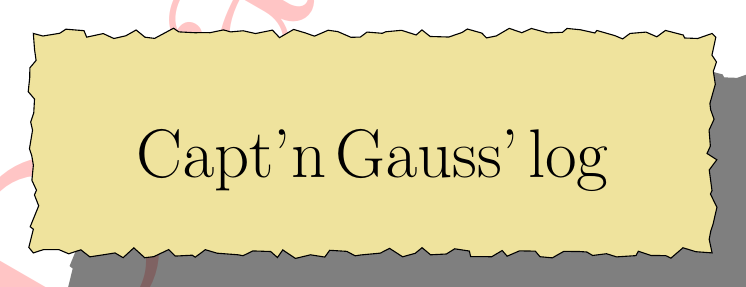
\begin{tikzpicture}[pencildraw/.style={ %
    decorate,
    decoration={random steps,segment length=4pt,amplitude=2pt}
    } %
]
\node[
preaction={fill=black,opacity=.5,transform canvas={xshift=.5cm,yshift=-.5cm}},
pencildraw,draw,fill=paper,text width=3in,inner sep=.5cm] 
{\begin{center}\Huge Capt'n Gauss' log \end{center}\vspace{.7cm} {\huge\context}};
\end{tikzpicture}}

\end{tabular*}

\vfill

\includegraphics[width=3in]{logoPirate.png}\hfill \includegraphics[width=2in]{bammLogo.png}


}


\begin{document}

\begin{context}

Land ahoy!

A treasure most fine is said to be hidden


on this mysterious island, 


by mazes of convoluted design.



Unlike any seen before,


with twists and turns that defy the laws of land and sea alike!

I could see that the mazes were indeed located on M\"obius bands, a surface with only one side and one edge. I knew that solving these mazes would require a deep understanding of the properties of this unusual surface, as well as a willingness to think outside the box.
\end{context}

\begin{directions}
  \begin{itemize}
    \item Choose a paper maze
\item Use scissors to cut along the marked lines 
\item Apply tape if needed
  \item Use a pencil to solve the maze
\end{itemize}
\end{directions}

\begin{example}
\end{example}

\begin{mathConnections}
  https://bartsnapp.github.io/Math-Outreach-Exhibits/mazes/
\end{mathConnections}
\end{document}
